
\documentclass{beamer}
\usepackage[UTF8]{ctex}
\usepackage{graphicx}
\usepackage[english]{babel}
\usepackage[T1]{fontenc}
\newcommand{\nb}{\nonumber}
\hypersetup{CJKbookmarks=true}
\usepackage{subfigure} %%图形或表格并排排列
\usepackage{colortbl,dcolumn}     %% 彩色表格
\setCJKfamilyfont{yh}{Microsoft YaHei}
\graphicspath{{figures/}}
\usetheme{Warsaw}
\usefonttheme[onlymath]{serif} 
%\usefoottemplate{\hbox{\tinycolouredline{structure!80!black} 
%{\color{white}{Hao Cao} \hfill{Analysis on optimizers}}}}

\setbeamertemplate{footline}[frame number]
\expandafter\def\expandafter\insertshorttitle\expandafter{%
	\insertshorttitle\hfill%
	\insertframenumber\,/\,\inserttotalframenumber}
\setbeamercovered{transparent}
%\usefoottemplate{\hbox{\tinycolouredline{structure!80!black} {\color{white}{Hao Cao} \hfill{week 1}}}}
\date{{\today}}



\begin{document}
\begin{frame}
	\title{基于隐马尔可夫模型的心梗阶段分析以及急性心梗事件预测}
	\author{
吴芷婧} % 显示作者
	\date{ }  % 显示日期
\titlepage
\end{frame}

\section{研究意义与文献综述}
\begin{frame}{目录}
\tableofcontents[sectionstyle=show/shaded,subsectionstyle=show/shaded/hide]
\end{frame}

\begin{frame}{研究意义}
\begin{itemize}
		\item 根据《中国心血管健康与疾病报告2019》,每年约有350万人死于心血管疾病,其中心肌梗死患病人数高达250万。
		\item 临床上心血管疾病特别是心梗后病人病情的快速演变具有时效性强,不确定性因素等特点,流行病学及回归分析已经不能很好的满足实际应用的需要。
		\item
		人口学信息、既往疾病史、家族疾病史等的简单样本数据已经不足以支撑对于病人病情演变的模拟。
		\item
        心梗后心血管意外事件预见性差,如何能够提早从微妙的状态波动中发现识别?
	\end{itemize}
\end{frame}


\begin{frame}{心梗后心脑血管事件早期预警及诊疗的医学研究进展}
\begin{itemize}
		\item 
    1998年发布的冠心病Framingham危险评分(FRS),采用的分析方法主要包括直接评分法和多元回归方法。
		\item
		欧洲国家建立起一种新的心血管疾病风险评估模型——Score模型。
		\item
		英国Qrisk心血管风险评估系统 (QRFSEARCH Cardiovascular Risk Algorithm),以Cox风险回归为主要分析方法。
		\item
		国内开展中国人群动脉粥样硬化性心血管疾病(ASCVD)发病风险预测研究(China-PAR),采用Cox风险比例回归模型。
	\end{itemize}
\end{frame}

\begin{frame}{数学建模及人工智能在医学应用上的发展及不足}
\begin{itemize}
		\item 
		在心梗发展问题上,缺乏刻画心梗发展阶段的指标。
		\item
		现阶段人工智能大数据方法可用于处理图片、音频等不同形式的多模态数据,但关于心梗后心脑血管事件的早期预警和诊疗还缺乏相应的研究。
	\end{itemize}
\end{frame}

\section{连续时间隐马尔可夫模型与心梗发展阶段}
\begin{frame}{目录}
\tableofcontents[sectionstyle=show/shaded,subsectionstyle=show/shaded/hide]
\end{frame}

\begin{frame}{HMM模型与心梗发展阶段}{VD-HMM模型(Variable-Duration Hidden Markov Model)}
\begin{itemize}
    \item 
    在传统HMM模型的基础上,加入不同心梗阶段的持续时长。
    
       \begin{figure}
  	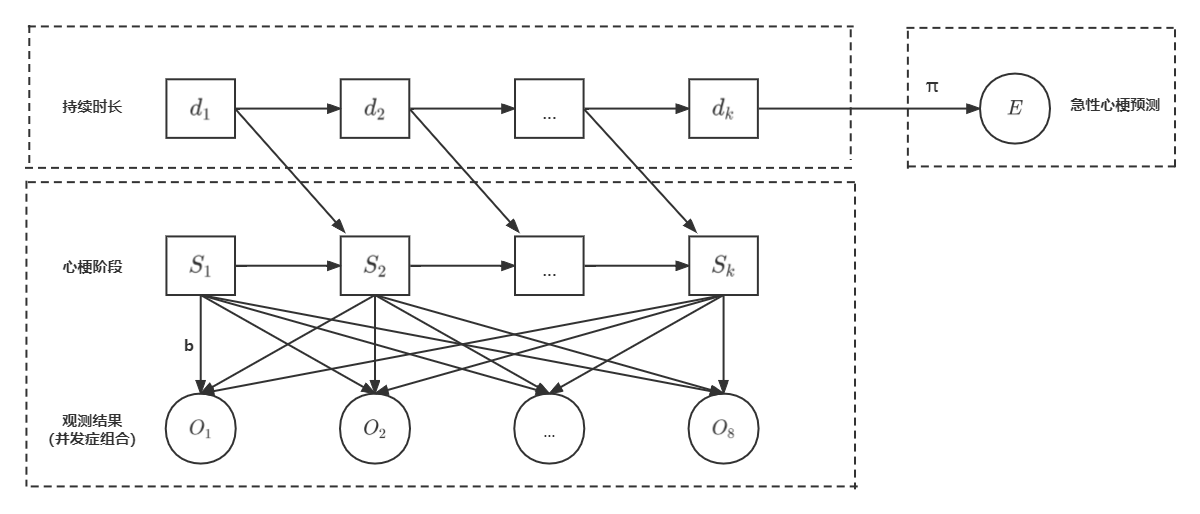
\includegraphics[width=10cm, height=5cm]{VDHMM模型}
    \end{figure}
\end{itemize}
\end{frame}

\begin{frame}{观测空间定义}
% \includegraphics[width=0.5\textwidth]{twc_m.png} 
\text{观测空间}
\begin{itemize}
    \item 
    从1266条诊断记录中,根据词频统计的方法,选择出出现频率最高的“胸闷”、“狭窄”、“胸痛”、“头晕”、“中段”、“呕吐”、“不适”、“恶心”八个并发症分词。
    \item
    将8个分词描述作为自变量输入、诊断结果作为因变量输出,分为非急性心梗(陈旧性心梗)与急性心梗,建立Logistic回归模型。
    \item 
    选择表现最好的“胸闷”“狭窄”“胸痛”三个分词作为观测空间。
\end{itemize}
% \includegraphics[width=0.5\textwidth]{twc.png} 
\end{frame}

\begin{frame}{观测空间定义}{分词回归结果}
    \begin{center}
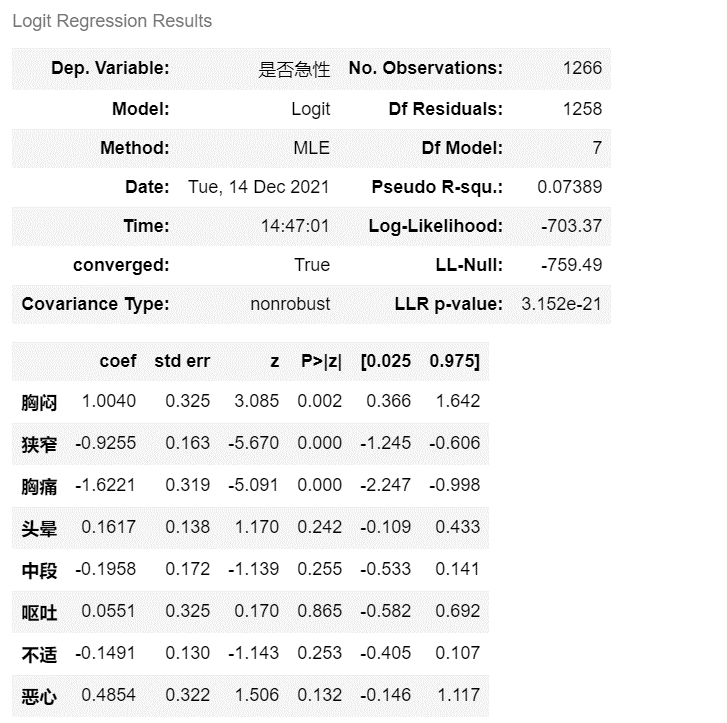
\includegraphics[width=0.6\textwidth]{分词回归.png}\\
\end{center}
\end{frame}

\begin{frame}{输出概率矩阵}
% \includegraphics[width=0.5\textwidth]{twc_m.png}

\begin{itemize}
\item
采用刻画离散型随机变量的多项式分布对输出概率矩阵进行参数化建模。
\begin{eqnarray*}
b_s(o_1,\cdots, o_M)
&=& P(O_1=o_1,\cdots,O_M=o_M|S=s) \nb \\
&=&
\left(\begin{array}{c}
n_s \\
o_{1} \cdots o_{M}
\end{array}\right) p_{1,s}^{o_{1}} \cdots p_{M,s}^{o_{M}}\nb\\
%&&\ for\ s\ \in \{1,\cdots, N\}.
% b_s(o_1,\cdots, o_M) 
\end{eqnarray*}

\item
待估参数
$$\{(p_{1,s},\cdots,p_{M,s})|s=1,\cdots,N\}$$

\end{itemize}
 
\end{frame}


\begin{frame}{转移概率}
\begin{itemize}
\item
转移概率函数
\begin{eqnarray*}
	 &&P(S_{i,j+1} = s'| S_{i,j} = s,d_j)\nb\\
	 &=&
	\begin{cases}
     	& p_{ss}(d_j,\Delta_{j,j+1},\sigma_{ij}) \qquad s'=s\\	
		& (1-p_{ss}(d_j,\Delta_{j,j+1},\sigma_{ij}))\Gamma_{ss'} \qquad s'\neq s
	\end{cases}
\end{eqnarray*}
其中
\begin{equation}
	\begin{aligned}
% 		& 
		p_{ss}(d_j,\Delta_{j,j+1},\sigma_{ij})
% 		\\	& 
		= logit^{-1}[\lambda_0^s + \lambda_1 log(1+d_j(s))\nb \\
		- log(\Delta_{j,j+1}) + \lambda_3\sigma_{ij}) ] \nb
	\end{aligned}
\end{equation}

\item
待估参数
$$\{(\lambda_0^s,\lambda_1,\lambda_3,\Gamma_{ss'})|\Gamma_{ss'}\in [0,1],\sum_{s'\neq s}^{N}\Gamma_{ss'}=1 ,s,s'=1,\cdots,N\}$$

\end{itemize}
 
\end{frame}



\section{模型参数估计}
\begin{frame}{目录}
\tableofcontents[sectionstyle=show/shaded,subsectionstyle=show/shaded/hide]
\end{frame}

\begin{frame}{离散时间隐马尔可夫模型与回归模型参数}
\begin{itemize}
    \item 离散时间隐马尔可夫模型参数\\
    $$\lambda=(N,M,\pi,A,B)$$
    \item 回归模型参数\\
    $$ logit(P(Y_{ij}=1|s_{ij},Z_{ij}))=w_0+\sum\limits_{s=1}^N w_s \mathcal{I}(s_{ij}=s)+w^T_Z\cdot Z_{ij}$$
\end{itemize}
\end{frame}

\begin{frame}{极大似然估计方法}
\begin{eqnarray}
    L(w,\lambda)&=&\sum\limits_{i=1}^{I} \log(P(o_{i1},\cdots,o_{iJ_{i}},y_{i1},\cdots,y_{iJ_{i}}~|~w,\lambda))\nb\\
    &=&\sum\limits_{i=1}^{I} \log(P(\bar{o_{i}},\bar{y_{i}}~|~w,\lambda))\nb\\
    &=&\sum\limits_{i=1}^{I} \log(P(\bar{y_{i}}~|~\bar{o_{i}},w,\lambda))
    + \sum\limits_{i=1}^{I}\log(P(\bar{o_{i}}~|~\lambda))\nb\\
    &\geq &\sum\limits_{i=1}^{I}\log(P(\bar{y_{i}}~|~\bar{s_i}^*,w))+\sum\limits_{i=1}^{I}\log P(\bar{s_i}^*~|~\bar{o_{i}},\lambda) \nb\\
    &+& \sum\limits_{i=1}^{I}\log(P(\bar{o_{i}}~|~\lambda)) \nb
\end{eqnarray}
\end{frame}

\section{模型参数估计结果}
\begin{frame}{目录}
\tableofcontents[sectionstyle=show/shaded,subsectionstyle=show/shaded/hide]
\end{frame}

\begin{frame}{基于并发症的急性心梗事件预测:基准模型,预测精度为71.88\%}
\begin{center}
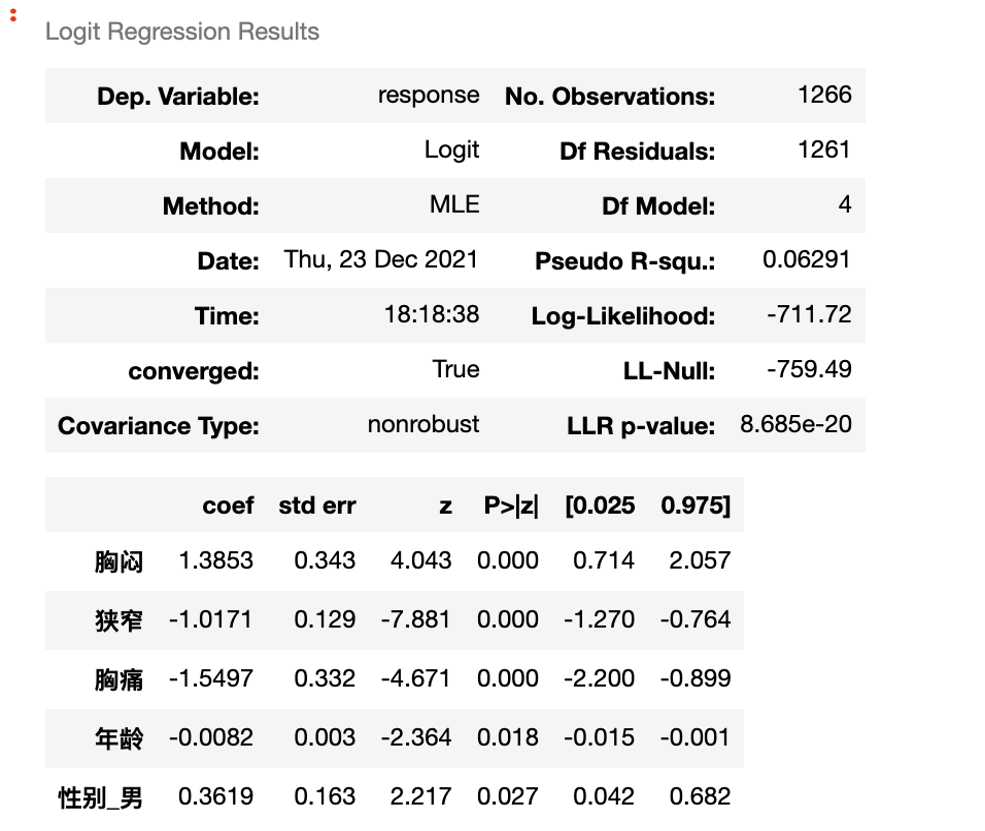
\includegraphics[width=0.6\textwidth]{LR_benchmark.png}\\
% \text{基于并发症的急性心梗事件预测,基准模型}\\
\end{center}
\end{frame}

\begin{frame}{选择状态空间元素个数为4}{隐马尔可夫模型参数}
    \begin{center}
    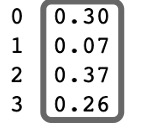
\includegraphics[width=0.1\textwidth]{初始分布4.jpeg}\\
    \text{表4:离散时间隐马尔可夫过程初始分布,N=4}\\
    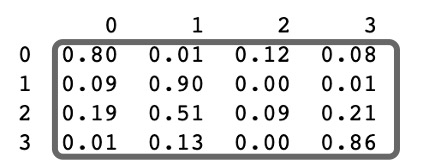
\includegraphics[width=0.3\textwidth]{转移概率矩阵4.jpeg}\\
    \text{表5:离散时间隐马尔可夫过程转移概率矩阵,N=4}\\
    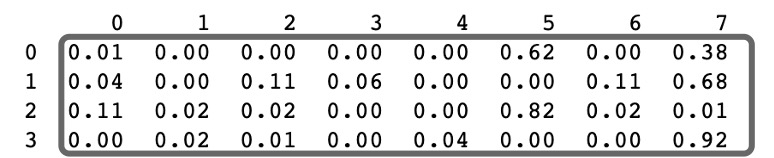
\includegraphics[width=0.6\textwidth]{输出概率矩阵4.jpeg}\\
    \text{表6:离散时间隐马尔可夫过程输出概率矩阵,N=4}
    \end{center}
\end{frame}

\begin{frame}{选择状态空间元素个数为4}{回归模型结果:预测精度为71.64\%}
    \begin{center}
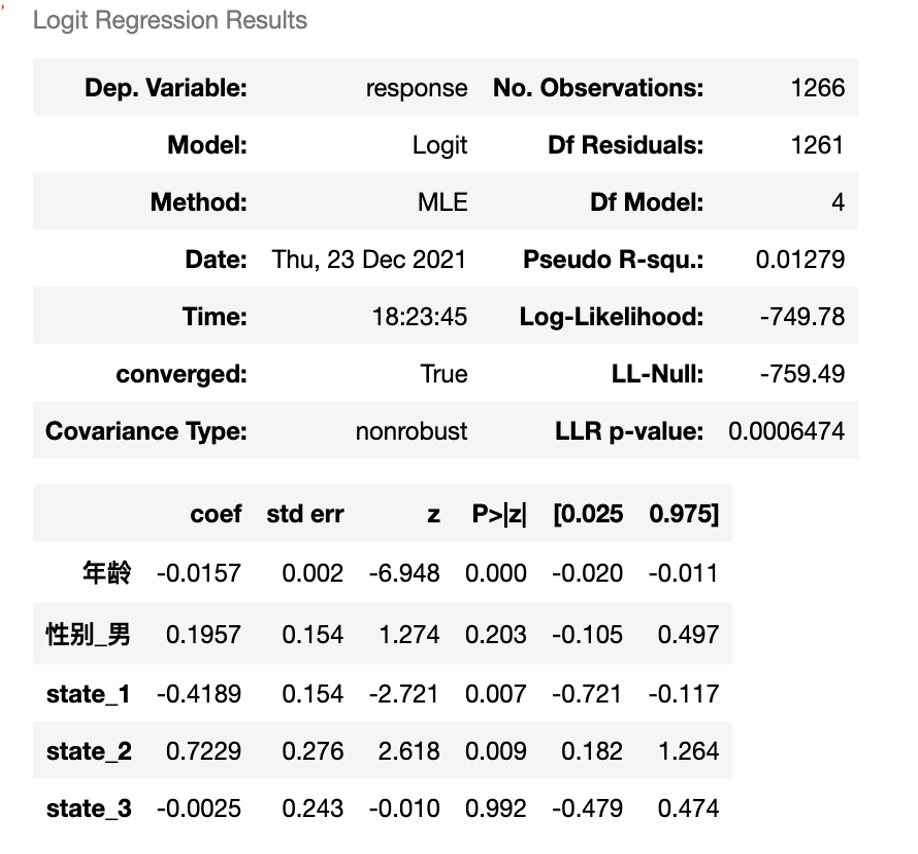
\includegraphics[width=0.6\textwidth]{LR_4.png}\\
    \end{center}
\end{frame}

\begin{frame}{选择状态空间元素个数为3}{回归模型结果:预测精度为71.56\%}
    \begin{center}
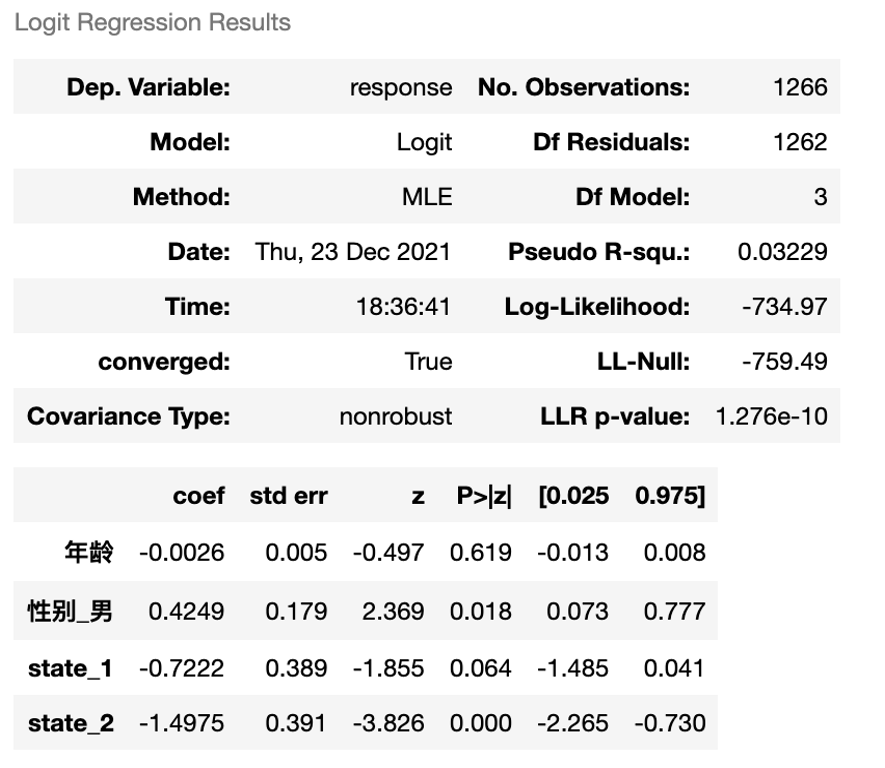
\includegraphics[width=0.6\textwidth]{LR_3.png}\\
    \end{center}
\end{frame}

\begin{frame}{选择状态空间元素个数为3}{隐马尔可夫模型参数}
    \begin{center}
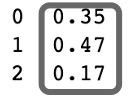
\includegraphics[width=0.15\textwidth]{初始分布3.jpeg}\\
\text{表8:离散时间隐马尔可夫过程初始分布,N=3}\\
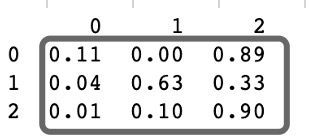
\includegraphics[width=0.4\textwidth]{转移概率矩阵3.jpeg}\\
\text{表9:离散时间隐马尔可夫过程转移概率矩阵,N=3}\\
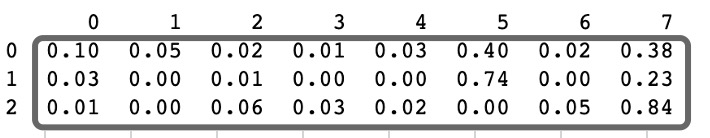
\includegraphics[width=0.8\textwidth]{输出概率矩阵3.jpeg}\\
\text{表10:离散时间隐马尔可夫过程输出概率矩阵,N=3}
    \end{center}
\end{frame}

\section{未来研究方向}
\begin{frame}{目录}
\tableofcontents[sectionstyle=show/shaded,subsectionstyle=show/shaded/hide]
\end{frame}

\begin{frame}{未来研究方向}
\begin{itemize}
    \item 除了并发症信息,我们计划纳入更多的危险因素信息(协变量)。
    \item 采用连续时间马氏过程分析心梗病人的心梗阶段发展。
    \item 在模型参数的估计方面,找到使似然函数本身最大化的一组参数。
\end{itemize}
\end{frame}

\begin{frame}{参考文献}
\begin{thebibliography}{99}
\bibitem CChristof Naumzik, Stefan Feuerriegel, Markus Weinmann. I Will Survive: Predicting Business Failures from Customer Ratings. Marketing Science, 2021.
\bibitem  
CKRISTIAN THYGESEN, JOSEPH S. ALPERT, ALLAN S. JAFFE, et al. Fourth Universal Definition of Myocardial Infarction (2018)[J].  Journal of the American College of Cardiology,2018,72(18):2231-2264.
\bibitem C胡盛寿,高润霖,刘力生,等.《中国心血管病报告2018》概要[J].中国循环杂志,2019,34(3):209-220.
\bibitem C中华医学会心血管病学分会,中华心血管病杂志编辑委员会.急性ST段抬高型心肌梗死诊断和治疗指南(2019)[J].中华心血管病杂志,2019,47(10):766 783.
\end{thebibliography}
\end{frame}

\begin{frame}{参考文献}
\begin{thebibliography}{99}
\bibitem
C中华医学会心血管病学分会,中华心血管病杂志编辑委员会.非ST段抬高型急性冠状动脉综合征诊断和治疗指南(2016)[J].中华心血管病杂志,2017,45(5):359 376.
\bibitem C黄广成,张远妮,邓光璞,等.急性心肌梗死患者住院费用的影响因素研究[J].中国卫生统计,2021,38(1):124-127.
\bibitem C马兴录,杨文文,冯云霞. 心血管疾病风险评估研究综述[J]. 计算机应用,2018,38(z2):111-114.
\bibitem 
CYANG, XUELI, LI, JIANXIN, HU, DONGSHENG, et al. Predicting the 10-Year Risks of Atherosclerotic Cardiovascular Disease in Chinese Population The China-PAR Project (Prediction for ASCVD Risk in China)[J].  Circulation: An Official Journal of the American Heart Association,2016,134(19):1430-1440. 
\end{thebibliography}
\end{frame}

\begin{frame}{Q\&A}
\tableofcontents
\end{frame}

\end{document}

